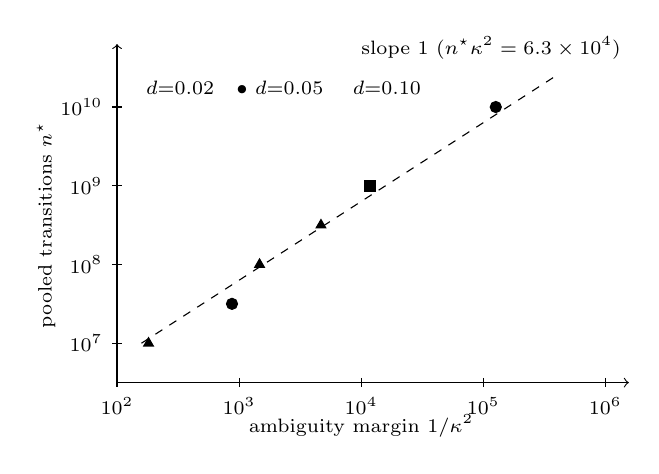
\begin{tikzpicture}[x=1cm,y=1cm,font=\scriptsize]
\draw[->] (0,0) -- (6.50,0);
\node at (3.10,-0.55) {ambiguity margin $1/\kappa^2$};
\draw[->] (0,0) -- (0,4.30);
\node[rotate=90] at (-0.9,2.00) {pooled transitions $n^\star$};
\draw (0.00,0.06) -- (0.00,-0.06) node[below] {$10^{2}$};
\draw (1.55,0.06) -- (1.55,-0.06) node[below] {$10^{3}$};
\draw (3.10,0.06) -- (3.10,-0.06) node[below] {$10^{4}$};
\draw (4.65,0.06) -- (4.65,-0.06) node[below] {$10^{5}$};
\draw (6.20,0.06) -- (6.20,-0.06) node[below] {$10^{6}$};
\draw (0.06,0.50) -- (-0.06,0.50) node[left] {$10^{7}$};
\draw (0.06,1.50) -- (-0.06,1.50) node[left] {$10^{8}$};
\draw (0.06,2.50) -- (-0.06,2.50) node[left] {$10^{9}$};
\draw (0.06,3.50) -- (-0.06,3.50) node[left] {$10^{10}$};
\draw[dashed] (0.31,0.50) -- (5.58,3.90);
\node[anchor=west] at (2.98,4.25) {slope $1$ ($n^\star\kappa^2=6.3\times10^{4}$)};
\node[mark size=2pt] at (3.21,2.50) {\pgfuseplotmark{square*}};
\node[mark size=2pt] at (4.81,3.50) {\pgfuseplotmark{*}};
\node[mark size=2pt] at (1.46,1.00) {\pgfuseplotmark{*}};
\node[mark size=2pt] at (2.59,2.00) {\pgfuseplotmark{triangle*}};
\node[mark size=2pt] at (1.81,1.50) {\pgfuseplotmark{triangle*}};
\node[mark size=2pt] at (0.40,0.50) {\pgfuseplotmark{triangle*}};
\node[anchor=north west,align=left] at (0.15,3.95) {$\blacksquare$ $d{=}0.02$\quad $\bullet$ $d{=}0.05$\quad $\blacktriangle$ $d{=}0.10$};
\end{tikzpicture}
